\begin{center}
    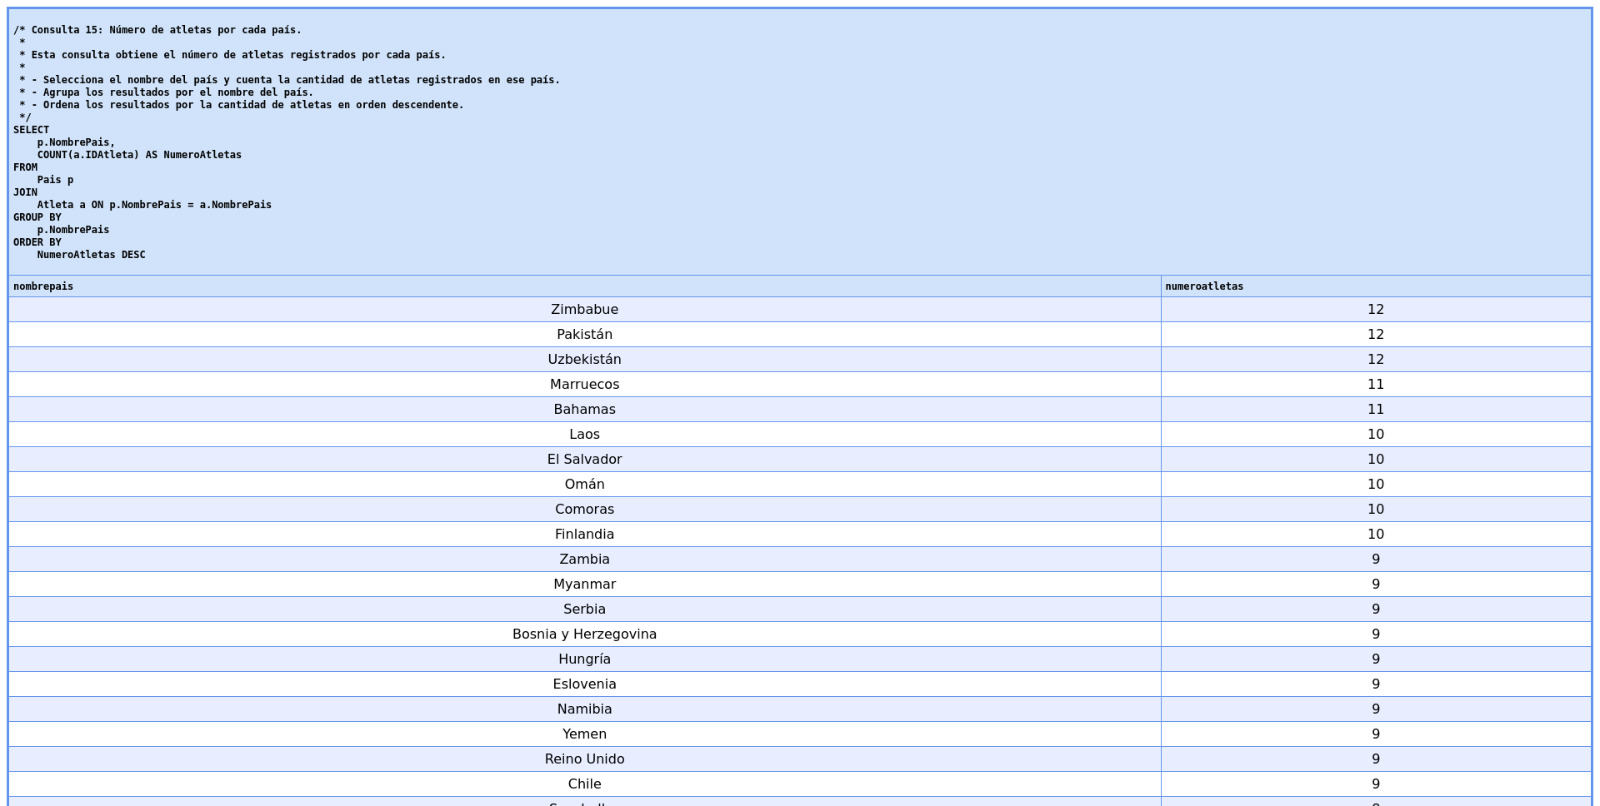
\includegraphics[width=16.5cm]{resources/Consulta15.jpeg} 
    
   Consulta 15. Número de atletas por cada país.
\end{center}

\textbf{Propósito de la consulta}

El objetivo de esta consulta es determinar cuántos atletas están registrados en cada país, proporcionando una visión general de la distribución de atletas a nivel internacional.

\textbf{Desglose de la consulta}

\begin{itemize}
   \item \textbf{Selección de columnas (\texttt{SELECT})}:
   \begin{itemize}
       \item \texttt{p.NombrePais}: Nombre del país de origen de los atletas.
       \item \texttt{COUNT(a.IDAtleta)}: Calcula el número total de atletas registrados en cada país. Esta columna se denomina \texttt{NumeroAtletas}.
   \end{itemize}

   \item \textbf{Tablas involucradas (\texttt{FROM} y \texttt{JOIN})}:
   \begin{itemize}
       \item \texttt{Pais (p)}: Contiene información sobre los países.
       \item \texttt{Atleta (a)}: Contiene información sobre los atletas.
       \item Se realiza un \texttt{JOIN} entre \texttt{Pais} y \texttt{Atleta} utilizando la relación \texttt{p.NombrePais = a.NombrePais}, que vincula a cada atleta con su país de origen.
   \end{itemize}

   \item \textbf{Agrupación de resultados (\texttt{GROUP BY})}:
   \begin{itemize}
       \item Los resultados se agrupan por \texttt{p.NombrePais}, para calcular el número de atletas registrados en cada país.
   \end{itemize}

   \item \textbf{Ordenamiento de resultados (\texttt{ORDER BY})}:
   \begin{itemize}
       \item Los resultados se ordenan en orden descendente (\texttt{DESC}) según la cantidad de atletas (\texttt{NumeroAtletas}), mostrando primero los países con más atletas registrados.
   \end{itemize}
\end{itemize}

\textbf{Análisis detallado}

\begin{enumerate}
   \item \textbf{Relación entre tablas:}
   \begin{itemize}
       \item La consulta utiliza la relación entre las tablas \texttt{Pais} y \texttt{Atleta} para asociar a cada atleta con su país de origen.
   \end{itemize}
   
   \item \textbf{Cálculo de atletas:}
   \begin{itemize}
       \item La función agregada \texttt{COUNT(a.IDAtleta)} cuenta el número de atletas registrados en cada país.
   \end{itemize}
   
   \item \textbf{Agrupación:}
   \begin{itemize}
       \item El uso de \texttt{GROUP BY} organiza los resultados por país, asegurando que cada país tenga un registro único con su conteo correspondiente de atletas.
   \end{itemize}
   
   \item \textbf{Ordenamiento:}
   \begin{itemize}
       \item El orden descendente por \texttt{NumeroAtletas} facilita la identificación de los países con mayor cantidad de atletas registrados.
   \end{itemize}
\end{enumerate}

\textbf{Consideraciones}

\begin{itemize}
   \item \textbf{Países sin atletas registrados:}
   \begin{itemize}
       \item Los países que no tienen atletas registrados no aparecerán en los resultados.
   \end{itemize}
   \item \textbf{Empates en cantidad de atletas:}
   \begin{itemize}
       \item Si dos o más países tienen el mismo número de atletas registrados, el orden relativo entre ellos no está definido. Se podría agregar un criterio adicional en el \texttt{ORDER BY}, como el nombre del país.
   \end{itemize}
\end{itemize}

\textbf{Utilidad de la consulta}

Esta consulta es útil para:
\begin{itemize}
    \item Analizar la distribución de atletas a nivel internacional.
    \item Identificar países con una alta o baja representación en términos de atletas registrados.
    \item Planificar estrategias para fomentar la participación en países con menor número de atletas.
    \item Evaluar la diversidad y alcance global del registro de atletas.
\end{itemize}
